\documentclass[aspectratio=169]{beamer}
\usepackage{color,amsmath}
\usepackage{subfigure}
\usepackage{booktabs}
\usepackage{framed}
\usepackage{comment}
\usepackage{url}

\newenvironment{rcases}
  {\left.\begin{aligned}}
  {\end{aligned}\right\rbrace}


%%%%%%%%%%%%%%%%%%%%%%%%%%
\title[]{Probability and non-probability sampling}
\author[]{Matthew J. Salganik\\Department of Sociology\\Princeton University}
\date[]{Summer Institutes in Computational Social Science\\2020
\vfill
\begin{flushleft}
{\scriptsize
The Summer Institutes in Computational Social Science is supported by grants from the Russell Sage Foundation and the Alfred P. Sloan Foundation.}
\end{flushleft}
\begin{flushright}

\includegraphics[width=0.1\textwidth]{figures/cc-by.png}
\end{flushright}
}
\begin{document}
%%%%%%%%%%%%%%%%%%%%%%%%%%
\frame{\titlepage}
%%%%%%%%%%%%%%%%%%%%%%%%%%
\begin{frame}

\begin{center}
\small{
\begin{tabular}{ l c c c}
           & Sampling & Interviews & Data environment\\
\hline
1st era & Area probability & Face-to-face & Stand-alone \\
2nd era & \parbox[t]{3cm}{\centering Random digital dial\\probability} & Telephone & Stand-alone \\
3rd era & \textcolor{blue}{Non-probability} & Computer-administered  & Linked \\
\end{tabular}
}
\end{center}

\end{frame}
%%%%%%%%%%%%%%%%%%%%%%%%%%%
\begin{frame}

\begin{center}
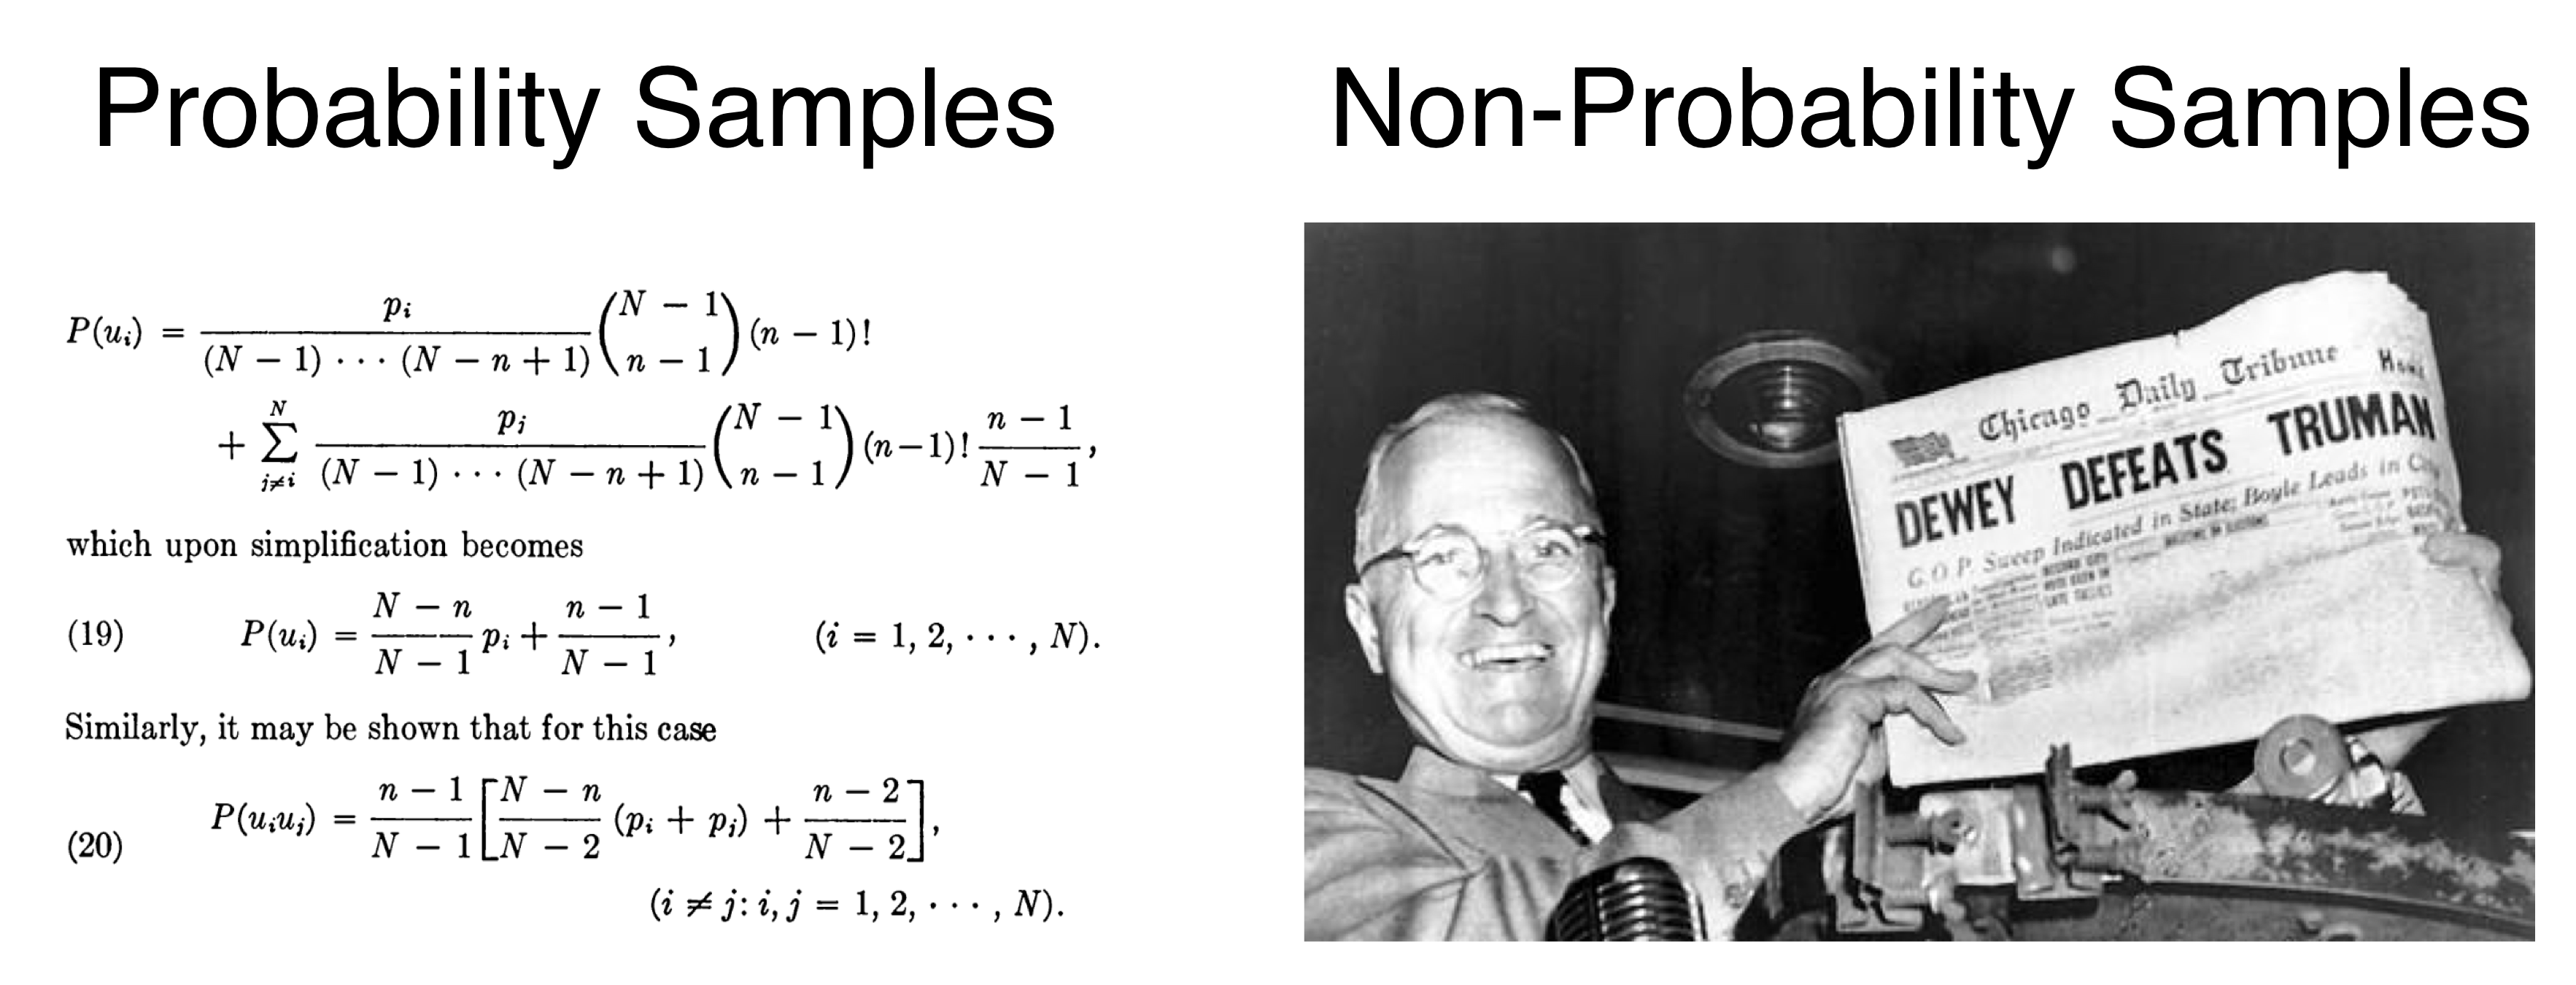
\includegraphics[width=\textwidth]{figures/prob_vs_nonprob_old}
\end{center}

\vfill
\TINY{\url{http://www.chicagotribune.com/news/nationworld/politics/chi-chicagodays-deweydefeats-story-story.html}}

\end{frame}
%%%%%%%%%%%%%%%%%%%%%%%%%%%
\begin{frame}

\begin{center}
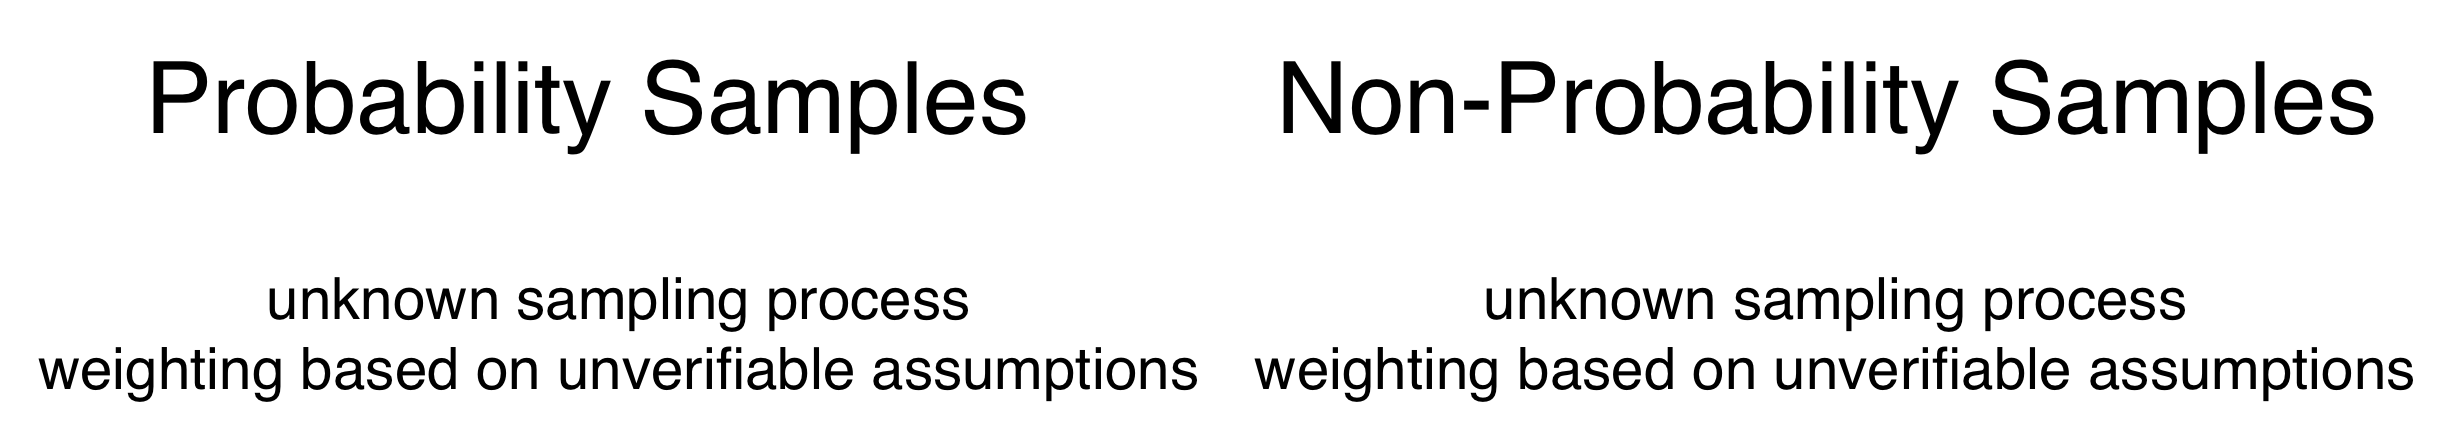
\includegraphics[width=\textwidth]{figures/prob_vs_nonprob_new}
\end{center}

\end{frame}
%%%%%%%%%%%%%%%%%%%%%%%%%
\begin{frame}

\begin{itemize}
\item Probability sample (roughly): every unit from a frame population has a known and non-zero probability of inclusion
\pause
\item Not all probability samples look like miniature versions of the population
\pause
\item But, with appropriate weighting, probability samples can yield unbiased estimates of the frame population
\end{itemize}

\end{frame}
%%%%%%%%%%%%%%%%%%%%%%%%%%
\begin{frame}

Main insight from probability samples:\\
\begin{itemize}
\item How you collect your data impacts how you make inference
\item Focus on properties of estimators not properties samples
\end{itemize}

\end{frame}
%%%%%%%%%%%%%%%%%%%%%%%%%%
\begin{frame}

Main idea and equation in sampling and estimation:
\begin{equation*}
\hat{\bar{y}} = \frac{\sum_{i \in s} y_i / \pi_i }{N}
\end{equation*}

where $\pi_i$ is person $i$'s probability of inclusion

\vfill

Sometimes called:
\begin{itemize}
\item Horvitz-Thompson estimator
\item $\pi$ estimator
\end{itemize}

\end{frame}
%%%%%%%%%%%%%%%%%%%%%%%%%
\begin{frame}

\begin{center}
{\Large Inference from probability samples in theory}
\end{center}

\begin{equation*}
\begin{rcases}
  \text{respondents} \\
  \text{known information about sampling}
\end{rcases}
\text{ estimates}
\end{equation*}

\pause

\vfill
\noindent\rule{\textwidth}{0.4pt}
\begin{center}
{\Large Inference from probability samples in practice}
\end{center}

\begin{equation*}
\begin{rcases}
  \text{respondents} \\
  \underbrace{\text{estimated information about sampling}}_{\text{auxiliary information + assumptions}}
\end{rcases}
\text{ estimates}
\end{equation*}

\pause 

\vfill
\noindent\rule{\textwidth}{0.4pt}

\begin{center}
{\Large Inference from non-probability samples}
\end{center}

\begin{equation*}
\begin{rcases}
  \text{respondents} \\
  \underbrace{\text{estimated information about sampling}}_{\text{auxiliary information + assumptions}}
\end{rcases}
\text{ estimates}
\end{equation*}

\end{frame}
%%%%%%%%%%%%%%%%%%%%%%%%%
\begin{frame}

\begin{equation*}
\hat{\bar{y}} = \frac{\sum_{i \in s} y_i / \hat{\pi}_i }{N}
\end{equation*}

where 
$\hat{\pi}_i = \frac{n_g}{N_g} \quad \forall \quad i \in g$ (estimated probability of inclusion)

\vfill

Requires:
\begin{itemize}
\item auxiliary information $(N_g)$
\item ability to place respondents in groups
\item assumptions
\end{itemize}

\end{frame}
%%%%%%%%%%%%%%%%%%%%%%%%
\begin{frame}

\begin{itemize}
\item Key to many adjustment methods is to use external information and make assumptions
\pause
\item If external information is incorrect or assumptions are wrong, then you can make things worse (but it usually seems to make things better)
\end{itemize}

\end{frame}
%%%%%%%%%%%%%%%%%%%%%%%%%%
\begin{frame}

Imagine that you want to estimate the average height of Princeton students.\\
\begin{itemize}
\item Assume 50\% are male and 50\% are female
\item You stand outside Lewis Library and recruit 60 Princeton students
\item Males (n= 20): Average height: 180cm
\item Females (n=40): Average heigh: 170cm
\end{itemize}
\textcolor{green}{What is your estimate of the average height? (think-pair-share)}

\end{frame}
%%%%%%%%%%%%%%%%%%%%%%%%%%
\begin{frame}

\begin{itemize}
\item sample mean = 173.3cm ($\frac{180 * 20 + 170 * 40}{20 + 40}$)
\pause
\item weighted estimate = 175cm ($180 * 0.5 + 170 * 0.5$)
\end{itemize}
\pause
How could this go wrong?

\end{frame}
%%%%%%%%%%%%%%%%%%%%%%%%%%
\begin{frame}

\begin{center}
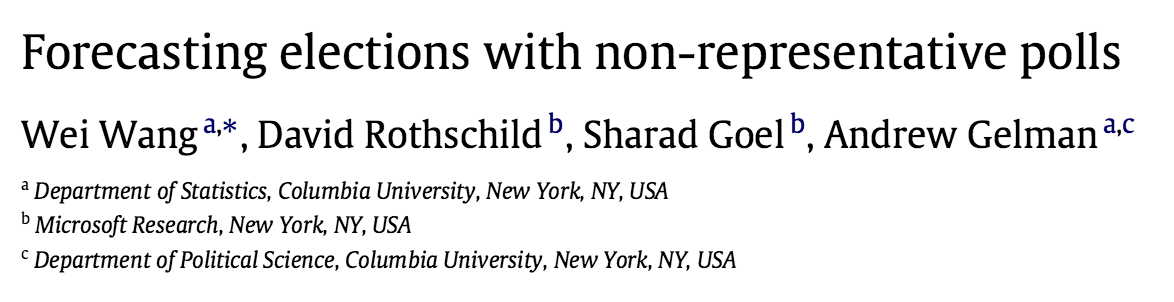
\includegraphics[width=\textwidth]{figures/wang_forecasting_2015_title}
\end{center}

\begin{center}

\includegraphics[width=0.5\textwidth]{figures/xboxlogo}
\end{center}

\end{frame}
%%%%%%%%%%%%%%%%%%%%%%%%%%%
\begin{frame}

\begin{center}
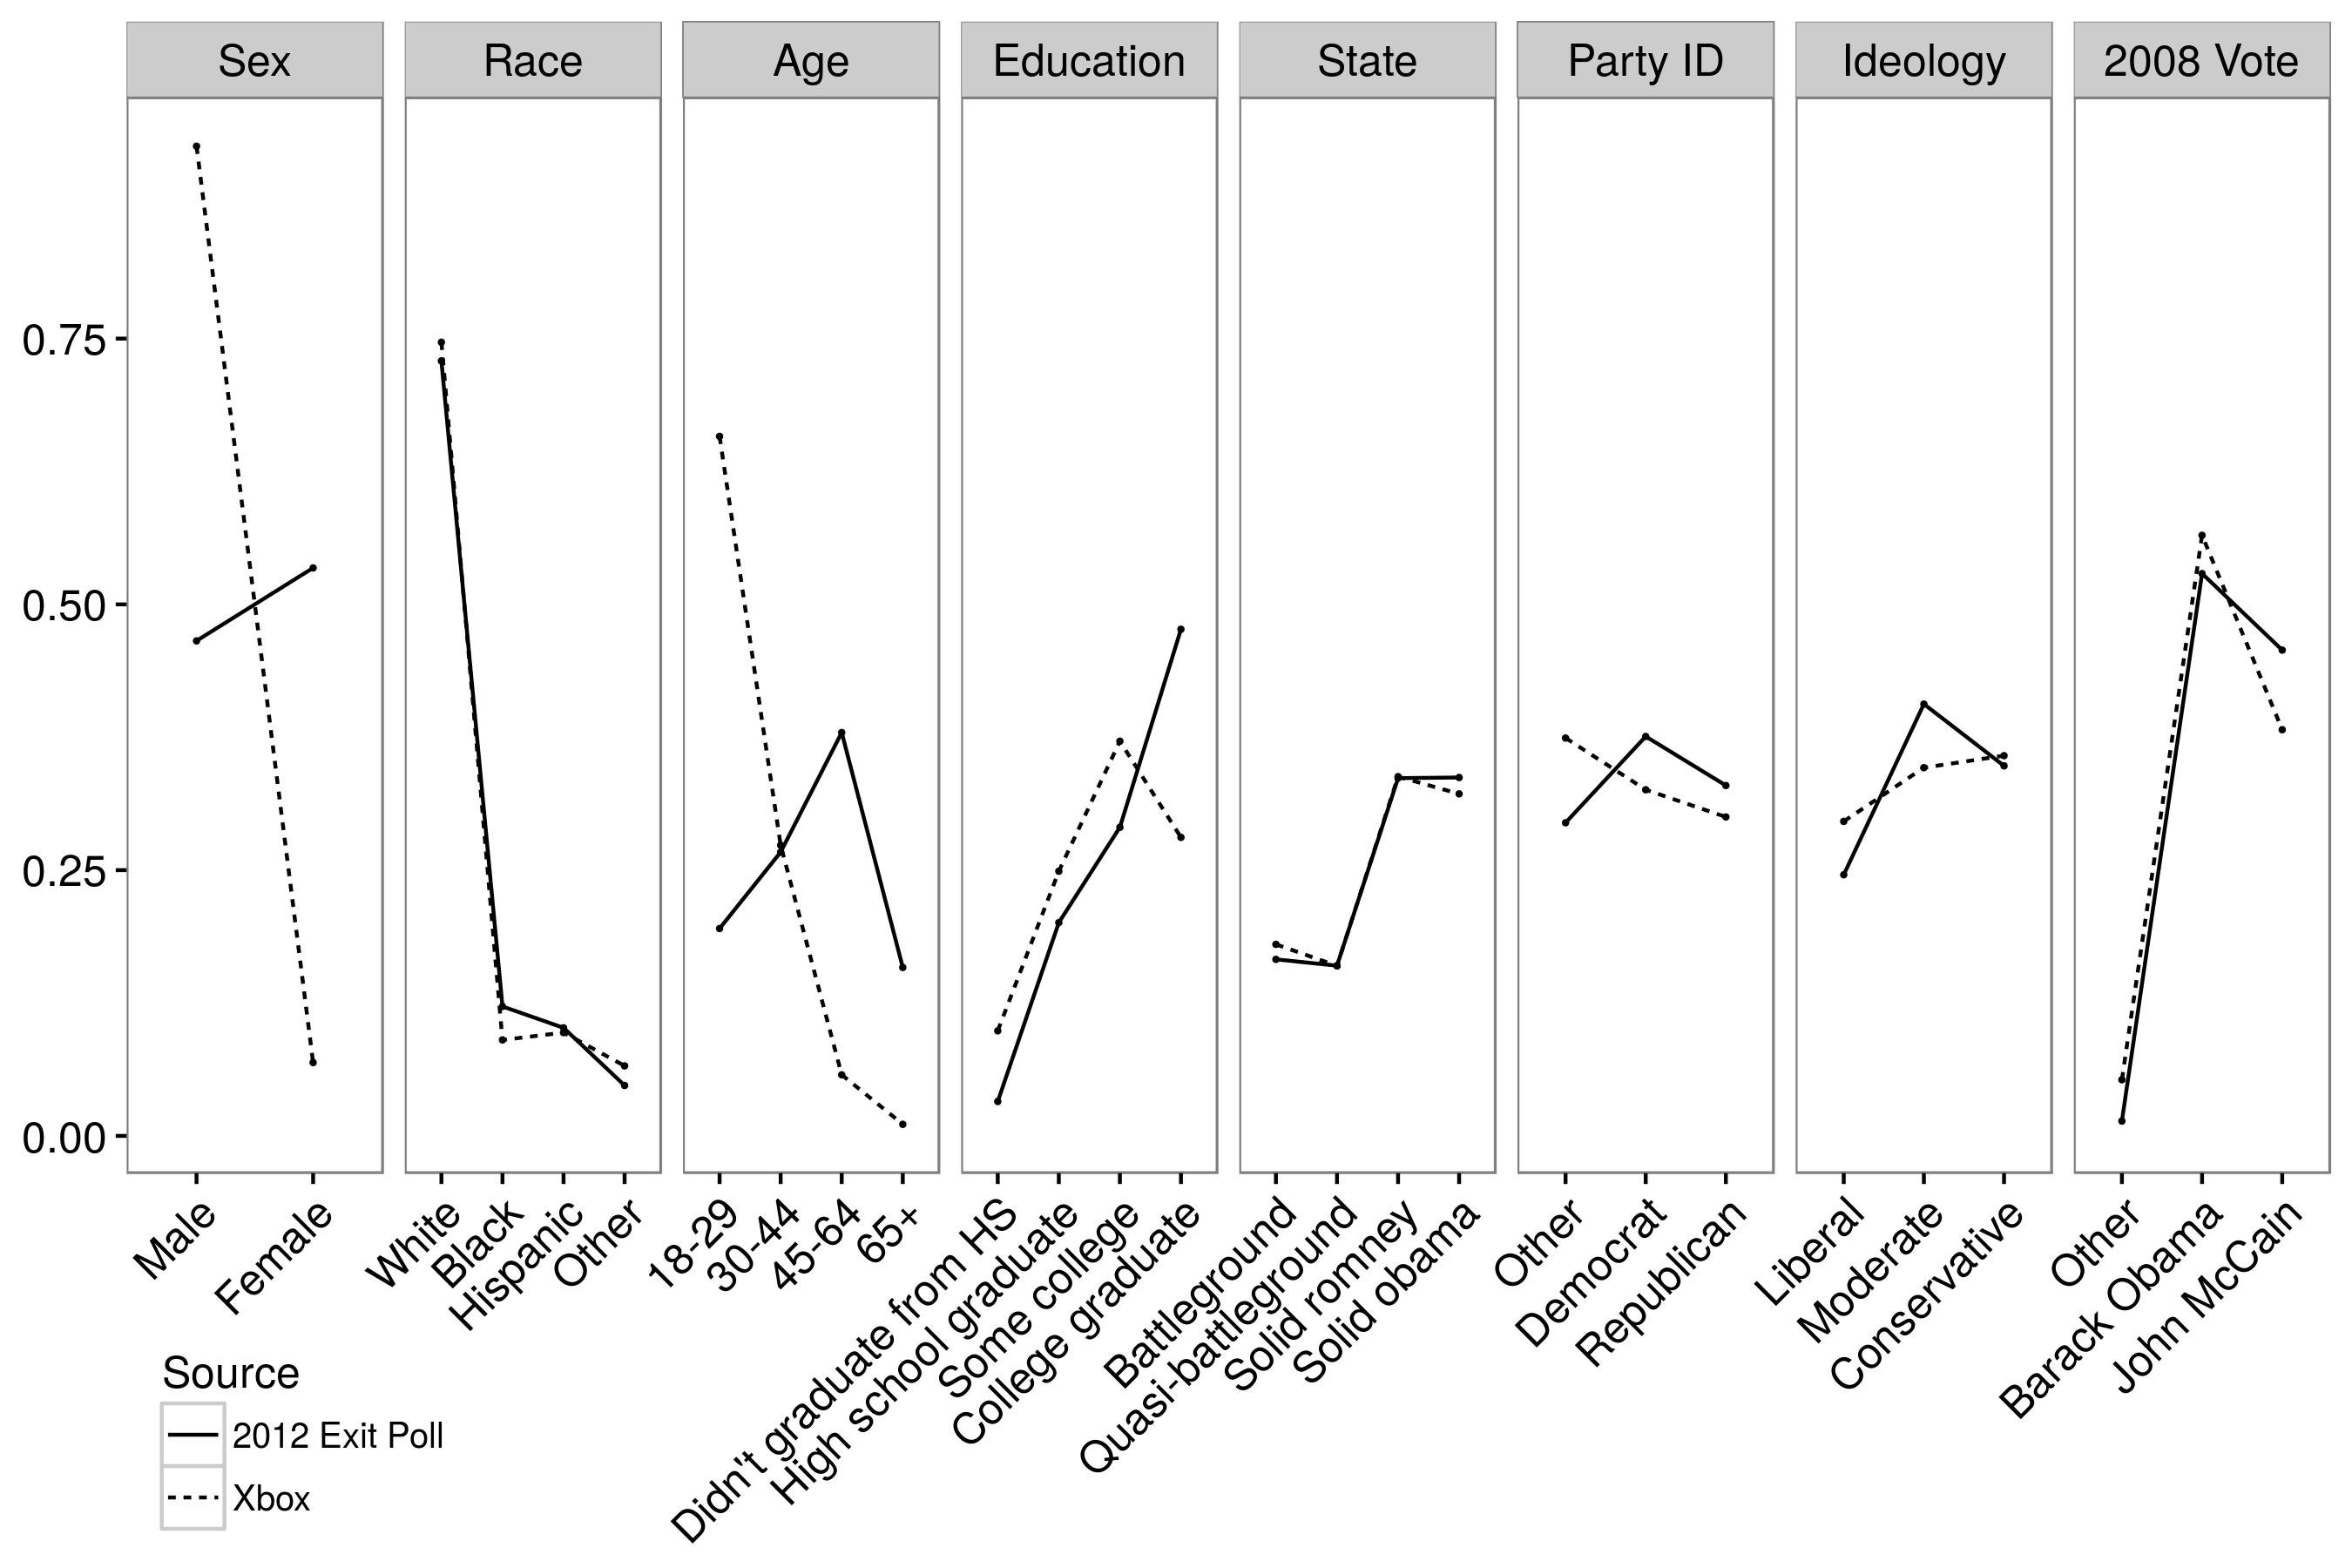
\includegraphics[width=0.6\textwidth]{figures/bitbybit3-7_wang_forecasting_2015_fig1}
\end{center}

\begin{itemize}
\item about 750,000 interviews
\item about 350,000 unique respondents
\end{itemize}

\end{frame}
%%%%%%%%%%%%%%%%%%%%%%%%%%%
\begin{frame}

\begin{center}
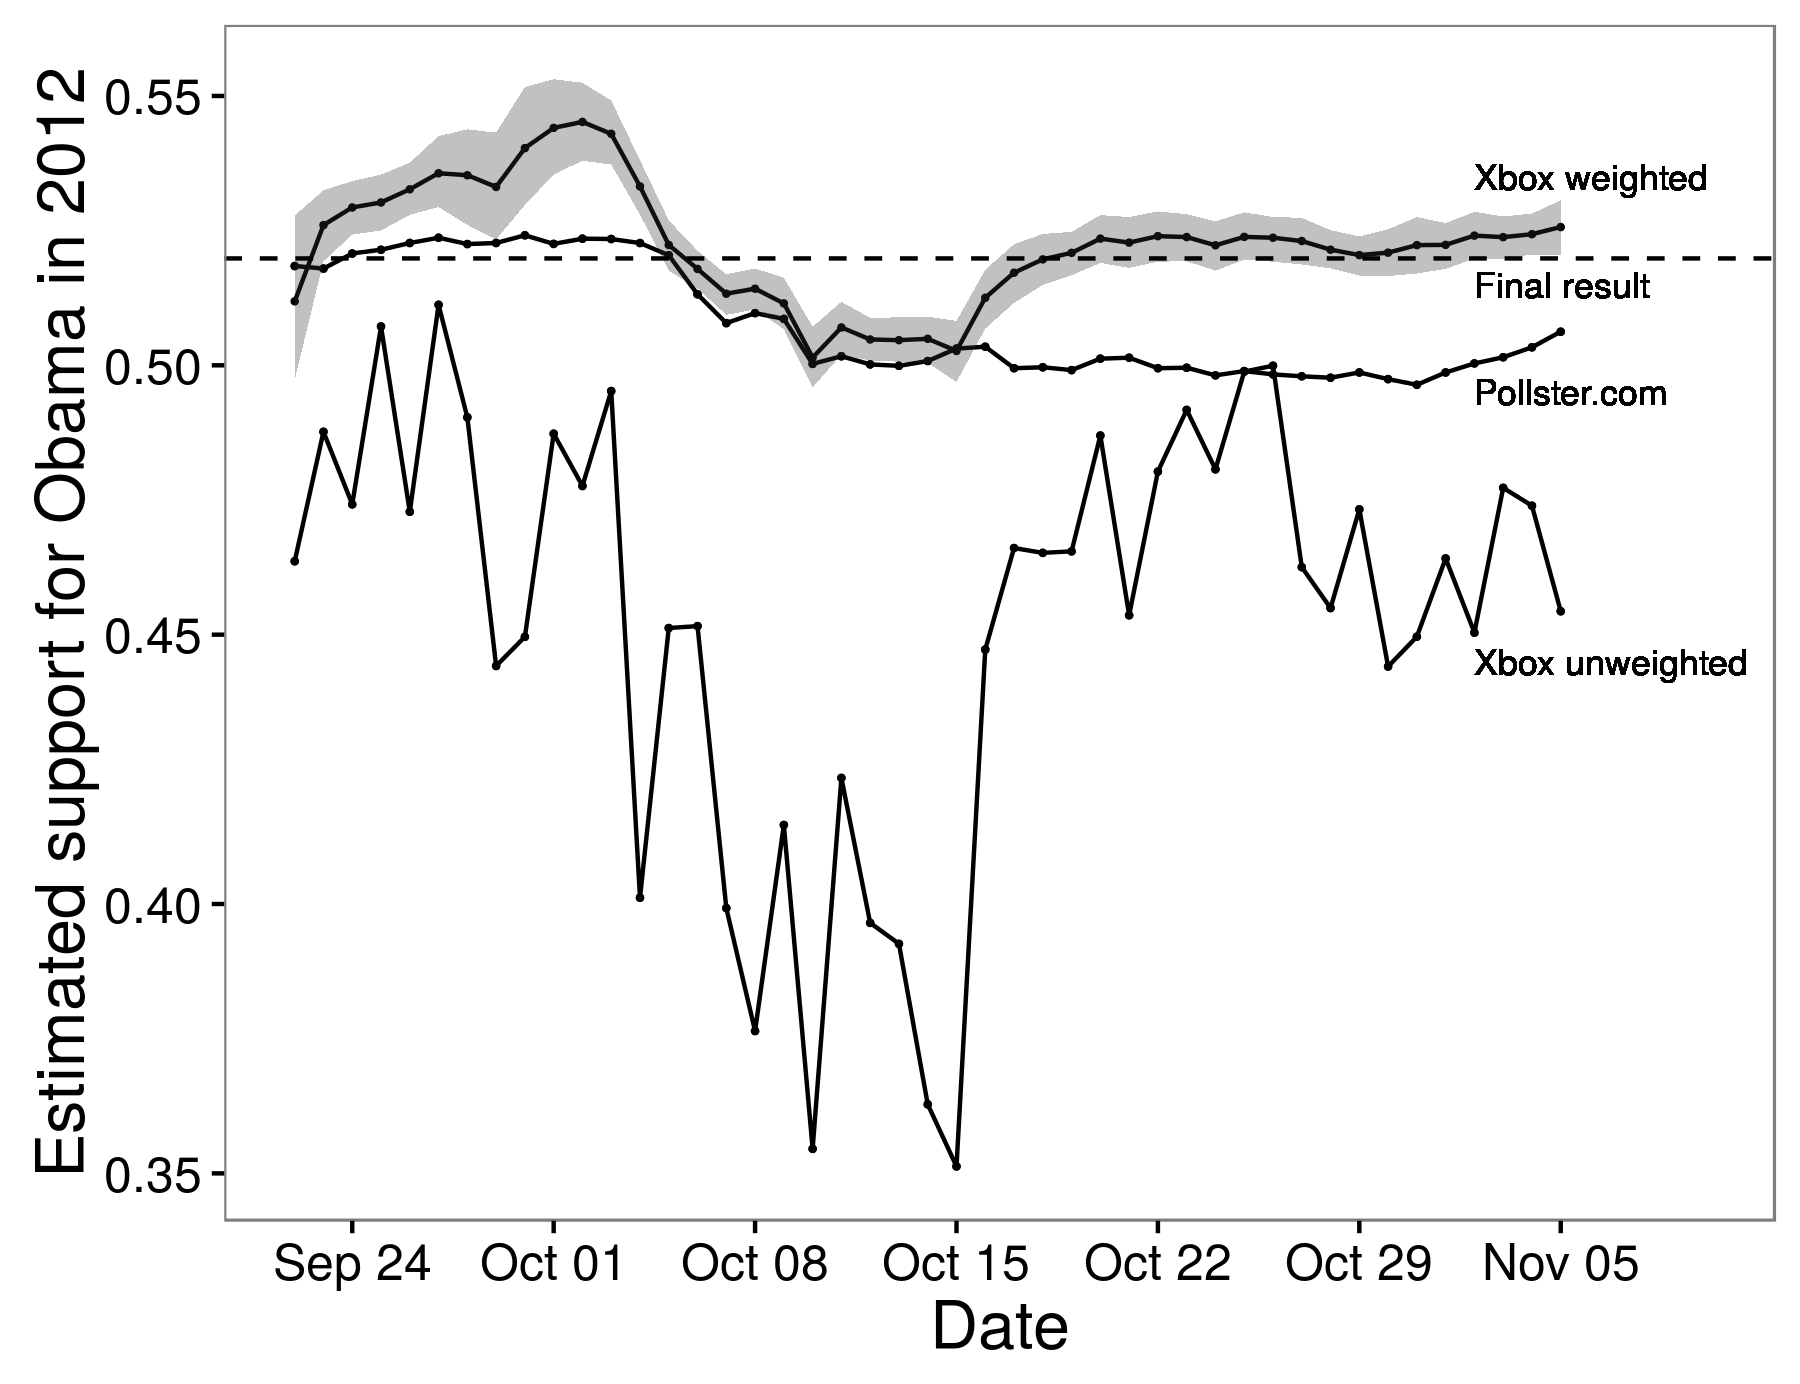
\includegraphics[width=0.8\textwidth]{figures/bitbybit3-8_wang_forecasting_2015_fig2_and_3}
\end{center}

\end{frame}
%%%%%%%%%%%%%%%%%%%%%%%%%%%
\begin{frame}

\begin{center}
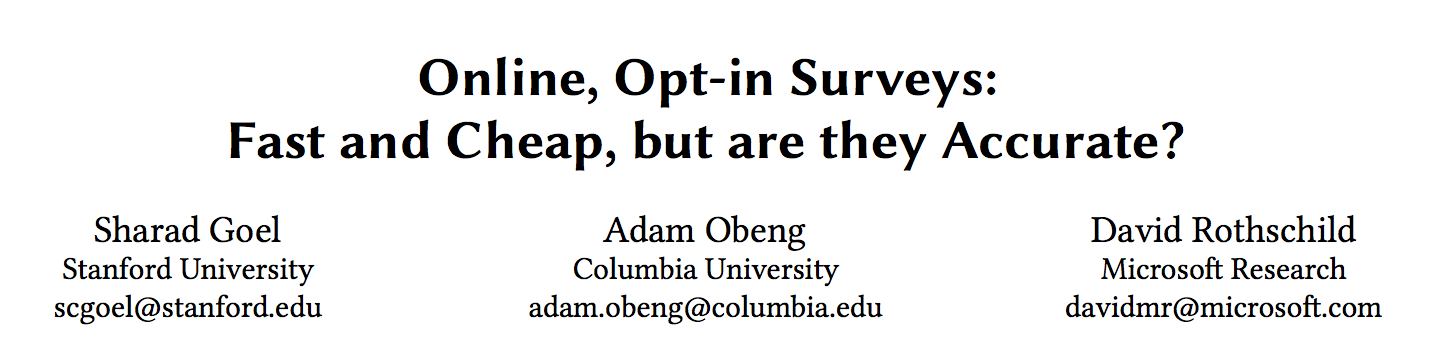
\includegraphics[width=0.9\textwidth]{figures/goel_online_2017_title}
\end{center}

\end{frame}
%%%%%%%%%%%%%%%%%%%%%%%%%%%
\begin{frame}

\begin{center}
\only<1>{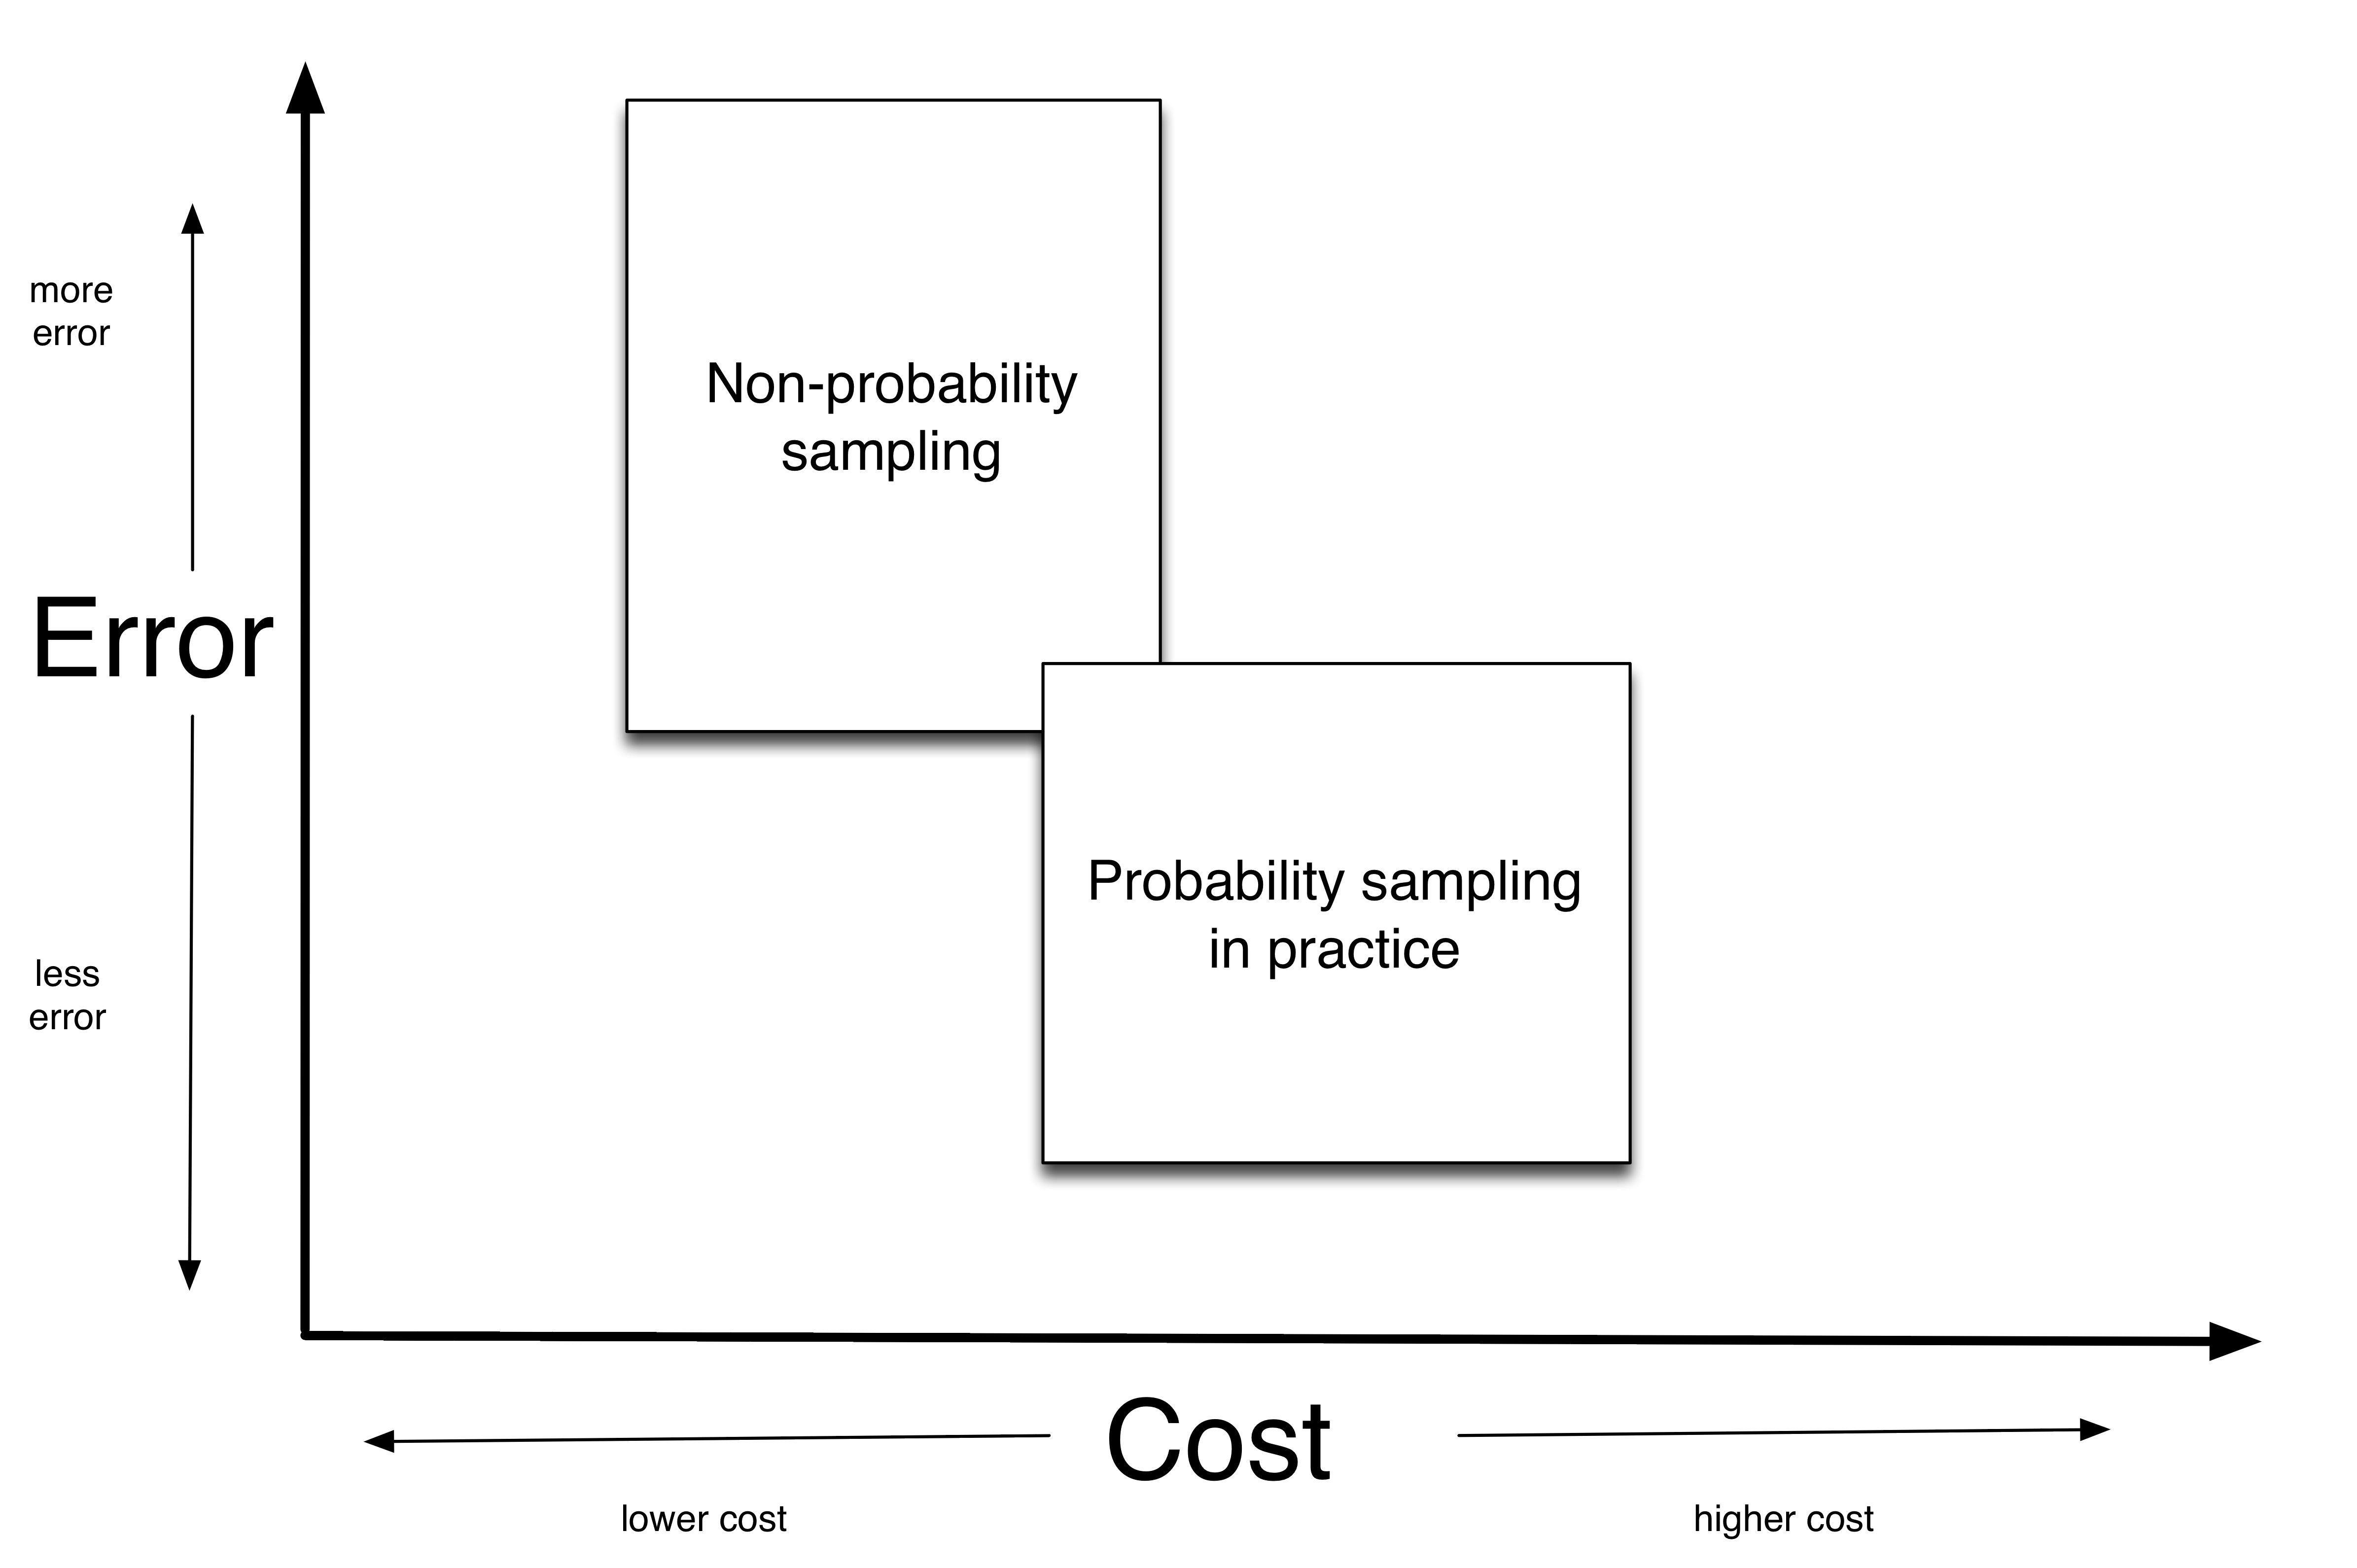
\includegraphics[width=0.8\textwidth]{figures/sampling_now}}
\only<2>{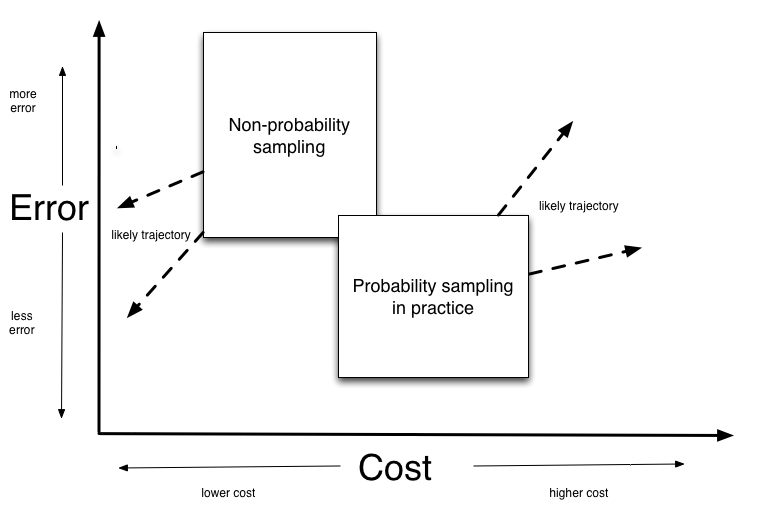
\includegraphics[width=0.8\textwidth]{figures/future_sampling}}
\end{center}

\end{frame}
%%%%%%%%%%%%%%%%%%%%%%%%%%%
\begin{frame}

Wrap-up:
\begin{itemize}
\item Samples don't need to look like mini-populations
\pause
\item Key to making good estimates is for estimation process to account for the sampling process
\pause
\item There is not a bright-line difference between probability sampling in practice and non-probability sampling
\pause
\item To learn more: Lohr (2009) or Sandal et al (2013)
\end{itemize}

\end{frame}
%%%%%%%%%%%%%%%%%%%%%%%%%%%

\end{document}
